% !Mode:: "TeX:UTF-8:Main"

\documentclass{article}
\usepackage[utf8]{inputenc} %probably not needed ...
\usepackage[T1]{fontenc}
\usepackage{geometry}
\geometry{papersize={128mm,96mm},margin=0.5cm} %\textwidth=11.8, \textheight=8.6
\usepackage[x11names,svgnames]{xcolor}
\usepackage{tikzducks}
\usetikzlibrary{shapes.geometric}
\pagestyle{empty}
\parindent=0pt
\begin{document}\definecolor{mygreen}{RGB}{149,150,90}\pagecolor{mygreen}
\begin{tikzpicture}[]

\duck[body=DarkGoldenrod1!20!AntiqueWhite1,beret,sunglasses]

 \begin{scope}
  \path[clip]
  \duckpathjacket;
  \node[anchor=south west] at (0,0){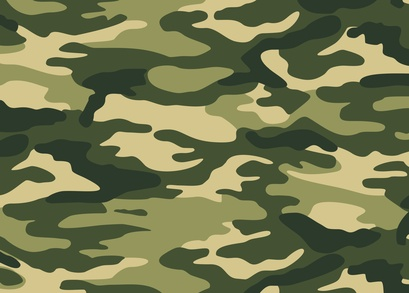
\includegraphics[width=3cm]{tarnmuster}};
 \end{scope}

\draw[thick] \duckpathjacket;

 \begin{scope}[rotate=-25]
  \draw[line width=1.5pt] (0.13,2.15) ellipse (0.5 and 0.17)
            (0.13,2.25) ellipse (0.55 and 0.17)
	        (0.13,2.4) circle (0.08);
 \end{scope}
 \begin{scope}[rotate=-25]
  \path[clip] (0.13,2.15) ellipse (0.5 and 0.17)
            (0.13,2.25) ellipse (0.55 and 0.17)
	        (0.13,2.4) circle (0.08);
  \node[anchor=south west] at (0,1){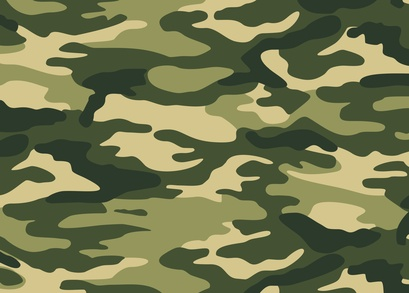
\includegraphics[width=3cm]{tarnmuster}};
 \end{scope}

\end{tikzpicture}
\end{document}